\chapter{Figuras, Tabelas e outros elementos}\label{chap:fundamentacaoTeorica}
Este capítulo apresenta a forma de incluir figuras, tabelas, equações, siglas e símbolos no documento, obtendo indexação automática em suas respectivas listas. A numeração sequencial de figuras, tabelas e equações ocorre de modo automático. Referências cruzadas são obtidas através dos comandos \verb#\label{}# e \verb#\ref{}#. Por exemplo, estou me referindo agora a introdução que corresponde ao  capítulo \ref{chap:introducao}.

\section{Figuras}
\label{sec:figuras}
Para incluir uma figura, use o ambiente \texttt{figure} e o comando \texttt{\textbackslash includegraphics}, como no exemplo a seguir:
\begin{figure}[!htb]
\centering
	
\includegraphics[width=0.3\textwidth]{./04-figuras/ifba2}
    \caption{Logo do IFBA}\vspace{-0.4cm}
    \fonte{\textcite{teste:2014}}
\label{fig:logoifba}
\end{figure}

A figura \ref{fig:logoifba} aparece automaticamente na lista de figuras. Para uso avançado de imagens no \LaTeX, recomenda-se a consulta de literatura especializada, como a \href{https://www.overleaf.com/learn/latex/Inserting_Images}{documentação de ajuda do Overleaf}.
\subsection{Figuras lado a lado}\label{figladoalado}
Abaixo segue um exemplo de como inserir figuras lado a lado:
\begin{figure}[H]
\centering
     \begin{subfigure}[b]{0.3\textwidth}
         \centering
         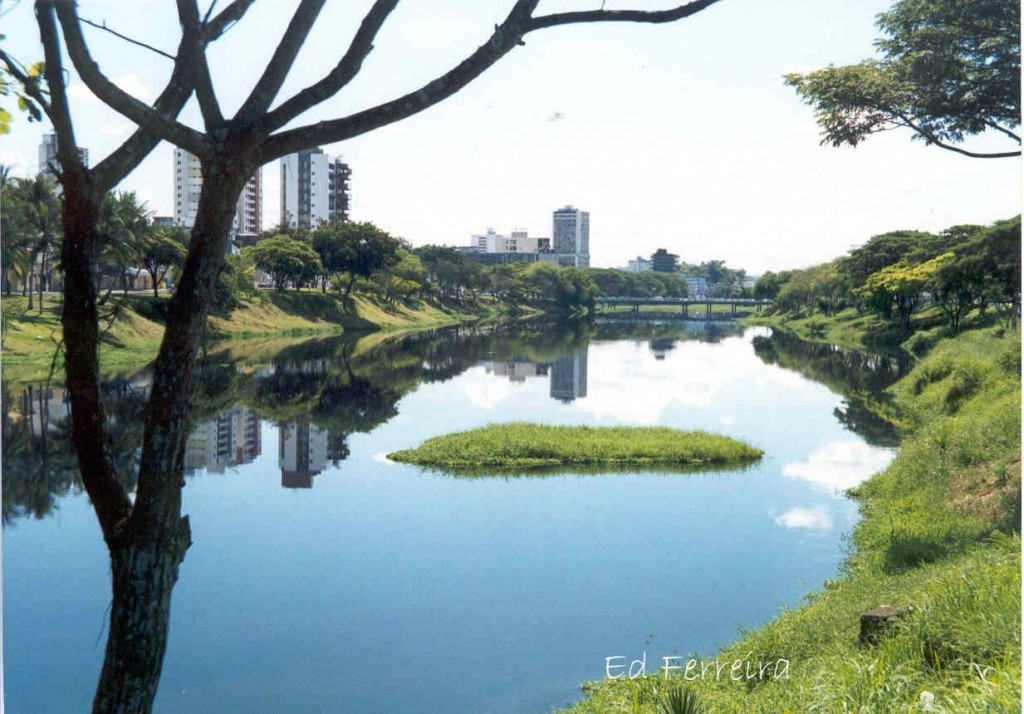
\includegraphics[width=\textwidth]{04-figuras/rc-adezanos}
         \caption{Rio Cachoeira em 2003}
         \label{fig:rc-adezanoss}
     \end{subfigure}\quad\qquad
     \begin{subfigure}[b]{0.3\textwidth}
         \centering
         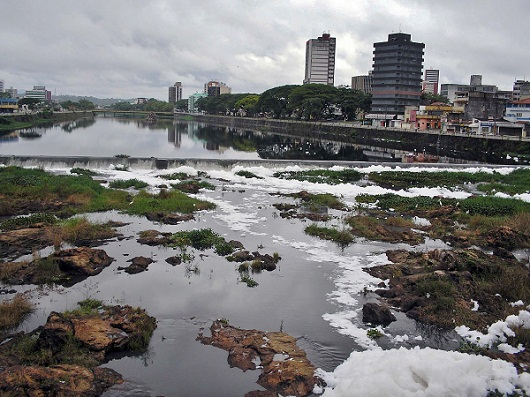
\includegraphics[width=\textwidth]{04-figuras/rc-atualmente}
         \caption{Rio Cachoeira em 2013}
         \label{fig:rc-atualmentee}
     \end{subfigure}
    \caption{Imagens comparando  o rio Cachoeira em 2003  e em 2013} \label{fig:estadorc}%\vspace{-0.6cm}
    \fonte{Pimenta Blog.BR, no endereço em $<$http://www.pimenta.blog.br/$>$}
\end{figure}

Para mais informações sobre como trabalhar com figuras em \LaTeX, consulte este \href{https://www.overleaf.com/learn/latex/Inserting_Images}{link do Overleaf}.

\section{Quadros e Tabelas}\label{sec:tabelas}
Para criar uma tabela, use o ambiente \texttt{table} e o ambiente \texttt{tabular}, como no exemplo a seguir:
\begin{table}[h]
  \caption{Exemplo de tabela}
  \centering
  \begin{tabular}{ccc}
    \hline
    \textbf{Item} & \textbf{Quantidade} & \textbf{Preço} \\
    \hline
    Maçã & 3 & R\$ 2,50 \\
    \hline
    Laranja & 2 & R\$ 1,80 \\
    \hline
    Pera & 4 & R\$ 3,20 \\
    \hline
  \end{tabular}
  \label{tab:exemplo}
\end{table}

Colocamos a Tabela \ref{tab:exemplo} no corpo do texto. podemos criá-la em um arquivo separado usando o ambiente \texttt{table} e o ambiente \texttt{tabular}, e em seguida chamá-la no texto utilizando o comando \verb|\input{arquivo}|. Dessa forma, o código fica mais organizado e fácil de editar. 

Segue  exemplos de tabelas criadas em arquivo separado:
\input{./05-tabelas/tabcorrelacao}

\input{./05-tabelas/tabteste}

Para quadros, segue um exemplo:
\input{./06-quadros/quacomparabd}

São referenciados da seguinte forma: Observe no quadro  \ref{qua:comparabd} … e na  tabela \ref{tab:correlacao} …

As tabela e quadros aparecem automaticamente na lista de tabelas conforme o título (\verb|caption|) dado. Informações sobre a construção de tabelas no LATEX podem ser encontradas  neste link de ajuda do Overleaf: \href{https://www.overleaf.com/learn/latex/Tables}{overleaf.com/learn/latex/Tables}.

Existem diversos sites que ajudam a gerar tabelas de maneira mais fácil para latex, entre os quais temos este: \href{https://www.tablesgenerator.com}{tablesgenerator.com}.
\section{Equações}\label{sec:equacoes}
Para apresentar equações em um documento \LaTeX, é possível utilizar o ambiente \texttt{equation}, que numerará as equações automaticamente e permitirá que sejam referenciadas ao longo do texto.

A transformada de Laplace é dada na equação \ref{eq:laplace}, enquanto a equação \ref{eq:dft} apresenta a formulação da transformada discreta de Fourier bidimensional.

\begin{equation}
X(s) = \int_{-\infty}^{\infty} x(t) , \text{e}^{-st} , dt
\label{eq:laplace}
\end{equation}

\begin{equation}
F(u, v) = \sum_{m = 0}^{M - 1} \sum_{n = 0}^{N - 1} f(m, n) \exp \left[ -j 2 \pi \left( \frac{u m}{M} + \frac{v n}{N} \right) \right]
\label{eq:dft}
\end{equation}

Uma equação mais simples como a ``fórmula de Bháskara'' segue abaixo:
\begin{equation}
    x=\frac{-b\pm\sqrt{b^2-4ac}}{2a}\label{eq:FormBhaskComp}
\end{equation}
A equação \eqref{eq:FormBhaskComp} pode ser separada em duas partes, conforme segue:\\
$\Delta=b^2-4ac$ e $x=-b\pm\sqrt{\Delta}$

É importante lembrar que, em equações com mais de uma linha, deve-se utilizar o ambiente \texttt{align} em vez de \texttt{equation}. Por exemplo:
\begin{align}
f(x) &= x^2 + 2x + 1 \
&= (x+1)^2
\end{align}

Nesse exemplo, a equação é dividida em duas linhas e alinhada pelo sinal de igualdade. 

Para aprender sobre ``modo matemático'', símbolos e equações em \LaTeX, consulte \href{https://pt.overleaf.com/learn/latex/Mathematical_expressions}{este endereço}.


\section{Algoritmos e códigos}
A maneira mais fácil de incluir códigos em \LaTeX~é criar um arquivo separado com a extensão correspondente ao programa para programar e  chamá-lo no corpo do texto com o comando \verb|\verbatiminput{nome_do_arquivo.extensão}|.

Por exemplo, vamos incluir um código do Método de Gauss para resolver sistemas lineares que está no diretório \verb|códigos|. Observe que usamos a extensão \verb|.m|, uma vez que o código foi programado em Octave que usa essa extensão.
\verbatiminput{07-Códigos/Met-Gauss.m}

Para gerar algoritmos ou Pseudocódigos dentro do próprio latex, você deve utilizar o pacote {\ttfamily algorithm2e} (já no preâmbulo). Para mais informações sobre como utilizar esse pacote, consulte a documentação disponível em \href{https://www.ctan.org/pkg/algorithm2e}{ctan.org/pkg/algorithm2e}.
